\documentclass[a4paper,12pt,oneside]{book}

\usepackage{ReadingNote}

%% other package
%\usepackage{coffeestains}
\usepackage{enumitem}
\setenumerate{itemsep=-1pt,parsep=0pt}
\setitemize{itemsep=-1pt,parsep=0pt}

\usepackage{url}
\usepackage{cleveref}
\usepackage{multicol}
\setlength{\columnsep}{5cm}

\usepackage{tikz,pgf}
\usetikzlibrary{arrows,positioning, graphs} % for drawing arrows in diagrams
\tikzset{
  candidate/.style={circle,draw=black, minimum size=.5cm,thick},
  ->,>=stealth',shorten >=1pt,shorten <=1pt,auto,node distance=1cm,semithick}

%% biblatex
\usepackage[backend=biber,style=apa]{biblatex}
\addbibresource{social_choice.bib}

%%%%%%Universal Macros%%%%%%%%



%%%%%%Particular Macros%%%%%%%
\newcommand{\weakor}{\mathcal{R}(A)} 
\newcommand{\linearor}{\mathcal{L}(A)}
\newcommand{\profile}{\mathbf{P}}
\newcommand{\N}{\mathbb{N}}
\newcommand{\pma}{>^\mu}
\newcommand{\ca}{\mathcal{C}(A)}
\newcommand{\condom}{\mathcal{D}_\textit{Condorcet}}
\newcommand{\scoringvec}{\mathbf{W}}
\newcommand{\Margin}{\textit{Margin}}
\newcommand{\splitnum}{\textit{Split}\#}
\newcommand{\cyclenum}{\textit{Cycle}\#}



\title{Notes for Social Choice}
\author{Stupid Icey}
\date{\today}


\begin{document}

\maketitle


\chapter*{Preface}
%\coffeestainA{0.9}{0.85}{-25}{5cm}{1.3cm}
\textbf{First Edition:}\\
A fucking stupid reading note of \textit{Handbook of Computational Social Choice} \parencite{Moulin2016} for fucking stupid me, and a lot of thanks to Eric Pacuit, a great teacher whose slides and handouts about Social Choice even makes me feel more stupid!\\
~\\
\noindent \textbf{Second Edition:}\\
The paper about \emph{Split cycle} by Wesley Holliday and Eric Pacuit \parencite{Holliday2020} is added. Thanks Gods I Am Still Alive!\\
Several parts ignored:
\begin{enumerate}
  \item Remark 3.13, about \emph{immunity to binary arguments} by \textcite{Heitzig2002} (formal argument theory).
  \item Remark 4.25, about \emph{choice function} and \emph{functional collective choice rule}.
  \item Remark 4.26, about \emph{expansion consistency} and \emph{reinforcement} and \emph{Condorcet component}(?). (Remark 3.11 in \textcite{Ding2023})
  \item Remark 5.25, about Ranked Pairs and \emph{clones}.
  \item Section 5.4.1, about \emph{Weighted Covering method}.
\end{enumerate}

\noindent And several parts which I really cannot understand\dots
\begin{enumerate}
  \item Section 5.4.2.2 (what is the \emph{proportion of profile} $\profile$?).
  \item Prop 5.43.
\end{enumerate}

\noindent And several questions:
\begin{enumerate}
  \item Definition B.2. Why we need such property\dots
  \item Why given a linear profile, the parity of all margins must be the same? Do other profiles have the same result?
\end{enumerate}
~\\
\noindent \textbf{Third Edition:}\\
Now reading Yifeng Ding's paper \parencite{Ding2023}.\\
Dingmen!!\\
~\\
Main topic: scfc in Section 8.


\tableofcontents

\part{Backgrounds and Preliminaries}
%% Chap1
\chapter{Arrow's Theorem}

\section{Basic Definition}

I combined the book with Eric's handout about Arrow's Theorem, which can be found on his website \parencite{Pacuit}.\\
~\\
We fix the following conventions:
\begin{itemize}
    \item $\weakor$ the set of all \textit{weak orders} $\succsim$ on $A$, i.e. the set of all binary relations on $A$ that are complete and transitive;
    \item $\linearor$ the set of all \textit{linear orders} $\succsim$ on $A$, which in addition are antisymmetric;
    \item $\succ$ the strict part of $\succsim$.
\end{itemize}

From finite sets of \textit{individuals} (or \textit{voters}, or \textit{agents}) and alternatives (or \textit{candidates}), respectively. Then we can get a \textit{profile}, from which we can construct a function assigning the profile to a \textit{social preference order}.

\begin{definition}[Profile]
    Let $N = \{1, \dots, n\}$ be a finite set of individuals, and $A$ be a finite set of alternatives. A \textit{profile} $\mathbf{P} = \linearor^n$, or to say, a function assigning to each $i \in N$ a linear order on $A$.
\end{definition}

For $a,b \in A$, let:
\begin{itemize}
    \item $\mathbf{P}(a,b) = \{i \in N\ |\ a \succ_i b\}$;
    \item $\mathbf{P}_{\upharpoonright\{a,b\}} = $ the function assigning to each $i \in N$ the relation $\succ_i \cap \;\{a,b\}^2$.
\end{itemize}

\begin{definition}[Social Welfare Function(SWF)]
    A \textit{social welfare function} (SWF) is a function $f: \; \mathbf{P} \to \weakor$. 
\end{definition}

We call the out come $\weakor$ as social preference order, and we write $\succsim$ for $f(\succsim_1,\dots, \succsim_n)$. Noted that here we allow ties in social preference order, but not in the individual preferences.\\
~\\
Then we introduce some properties about SWF, where the first two is considered reasonable by lots of people, while the last is not.

\begin{itemize}
    \item \textit{weakly Paretian:} For all $a,b \in A$, if $\mathbf{P}(a,b) = N$, i.e. $a \succ_i b$ for all $i \in N$, then $a \succ b$;
    \item \textit{independent of irrelevant alternatives (IIA):} For all $\mathbf{P},\mathbf{P'} \in \mathrm{Dom}(f)$ and $a ,b \in A$, if $\mathbf{P}_{\upharpoonright\{a,b\}} = \mathbf{P'}_{\upharpoonright\{a,b\}}$, then $a \succ b$ iff $a \succ' b$;
    \item \textit{dictatorship:} There is an $i^\star \in N$ s.t. for all $a,b \in A$, if $a \succ_{i^\star} b$, then $a \succ b$.
\end{itemize}
~\\
We hope that our SWF is both weakly Paretian and IIA, but not be a dictatorship. There shouldn't be a dictator in our voter-group. However, Arrow's Theorem just tell us that is impossible.

\begin{theorem}[Arrow's Theorem]
    When there are three or more alternatives, then every SWF that is weakly Paretian and IIA must be a dictatorship.
\end{theorem}

\section{Proof of Arrow's Theorem}

Here we first introduce the concept of \textit{decisive coalition}.

\begin{definition}
    A coalition $C \subseteq N$ of individuals is called a \textit{decisive coalition} for alternative $a$ versus alternative $b$, if for all $\mathbf{P} \in \mathrm{Dom}(f)$, $C \subseteq \mathbf{P}(a,b)$ implies $a \succ b$.
\end{definition}

We call $C$ \textit{weakly decisive} for $a$ vs. $b$, if at least $C = P(a,b)$ implies $a \succ b$. \\
\indent Notice that an SWF is weakly Paretian is the same as to say that the grand coalition $N$ is decisive, and $f$ is dictatorial is the same as to say that there exists a singleton that is decisive.\\
~\\
\textit{Sketch of proof:} Suppose that $|A| \geq 3$ and let $f$ be any SWF that is weakly Paretian and IIA. Since $f$ is weakly Paretian, the individual-set $N$ is a decisive coalition. First we show that for all weakly decisive coalition for $a$ vs.$\, b$, it's also decisive for all pairs of alternatives. Thus $N$ is decisive for all pairs. Then we split $N$ into two nonempty subsets again and again, until we obtain a coalition which is a singleton. We show that every time we split a decisive coalition up, one of the subsets remains decisive. Thus the final singleton we got from spliting $N$ up is decisive, say, a dictator.

\begin{lemma}[Contagion (or Field Expansion)]
    \label{Contagion}
    If $C$ is weakly decisive for $a$ vs. $b$, then $C$ is decisive for all pairs of alternatives.
\end{lemma}

\begin{proof}
    Let $\mathbf{P} \in \mathrm{Dom}(f)$ and $C$ is a coalition s.t. $C \subseteq \mathbf{P}(a',b')$ for arbitrary alternatives $a',b'$ and $C$ is weakly decisive for $a$ vs.$\, b$. Our goal is to show that $C$ is decisive for $a' \mbox{ vs.}\,b'$.\\
    W.L.O.G. let $a,b,a',b'$ be mutually distinct (the other cases are similar). Consider a special profile $\mathbf{P'}$ s.t. $\mathbf{P'}_{\upharpoonright\{a',b'\}} = \mathbf{P}_{\upharpoonright\{a',b'\}}$, $a' \succ_i a \succ_i b \succ_i b'$ for all $i \in C$, $a' \succ_j a ,\  b \succ_j b'$ and $b \succ_j a$ for all $j \in N \backslash C$.\\
    Since $C$ is weakly decisive for $a \mbox{ vs.}\, b$ and $C = \mathbf{P'}(a,b)$, we have $a \succ_\mathbf{P'} b$. Since $\mathbf{P'}(a',a) = \mathbf{P'}(b,b') = N$, from $f$ being weakly Paretian, $a' \succ_\mathbf{P'} a$ and $b \succ_\mathbf{P'} b'$. Since $\weakor$ is transitive, we have $a' \succ_\mathbf{P'} a \succ_\mathbf{P'} b \succ_\mathbf{P'} b'$.\\
    Since $f$ is IIA and $\mathbf{P'}_{\upharpoonright\{a',b'\}} = \mathbf{P}_{\upharpoonright\{a',b'\}}$, we have $a' \succ b'$. Thus $C$ is decisive for $a' \mbox{ vs.}\, b'$.
\end{proof}

\begin{lemma}[Splitting (or Group Contraction)]
    \label{Splitting}
    For any $C \subseteq N$ with $|C| \geq 2$ that is decisive, there is nonempty sets $C_1, C_2 \subseteq C$ with $C_1 \cup C_2 = C$ and $C_1 \cap C_2 = \emptyset$ s.t. one of $C_1 \mbox{ and }C_2$ is decisive for all pairs as well.
\end{lemma}

\begin{proof}
    Recall that $|A| \geq 3$. Let $C$ be a decisive coalition s.t. $|C| \geq 2$. Consider a profile $\mathbf{P}$ in which everyone ranks alternatives $a,b,c$ in the top three positions. Furthermore, $a \succ_i b \succ_i c$ for all $i \in C_1$, $b \succ_j c \succ_j a$ for all $j \in C_2$ and $c \succ_k a \succ_k b$ for all $k \in N \backslash C$, where $C = C_1 \cup C_2$.\\
    As $C$ is decisive, we have $b \succ c$. By the completeness of $\weakor$, either $a \succ c$ or $c \succsim a$. \\
    We conseder two cases.
    \begin{itemize}
        \item[\textit{Case 1:}] $a \succ c$: $\mathbf{P}(a,c) = C_1$. Since $f$ is IIA, for any profile $\mathbf{P'} \in \mathrm{Dom}(f)$ s.t. $\mathbf{P'}_{\upharpoonright\{a,c\}} = \mathbf{P}_{\upharpoonright\{a,c\}}$, we have $C = \mathbf{P'}(a,c)$ implies $a \succ_\mathbf{P'} c$. Thus $C$ is weakly decisive for $a \mbox{ vs.} \, b$. By \cref{Contagion}, $C$ is decisive for all pairs.
        \item[\textit{Case 2:}] $c \succsim a$: By transitivity of $\weakor$, $b \succ a$. With $\mathbf{P}(b,a) = C_2$, analogously we can conclude that $C_2$ is weakly decisive for $b \mbox{ vs.} \, a$, thus decisive for all pairs.
    \end{itemize}
\end{proof}

\section{Another Version of Proof}

In this part, I will give another version of Arrow's Theorem, which is mentioned by Eric Pacuit. The main difference between the two versions is the part after \cref{Contagion}.

By \cref{Contagion}, let $\mathcal{D} = \{C \ |\ C \mbox{ is decisive }\}$. Then
\begin{itemize}
    \item $\mathcal{D} \neq \emptyset$, since $N \in \mathcal{D}$;
    \item Since $N$ is finite, there is a minimal $C \in \mathcal{D}$, i.e. there is no $C' \in \mathcal{D}$ s.t. $C' \subsetneq C$.(?)
\end{itemize}

Now we prove the following:
\begin{lemma}
    \label{minimal}
    Let $f$ be an SWF and $\mathcal{D} =\{C\ |\ C \mbox{ is decisive }\}$. If $C,C' \in \mathcal{D}$ are minimal, then $C = C'$.
\end{lemma}

\begin{proof}
    Let $\mathcal{D}$ be the set of all decisive coalition for SWF $f$ with $C,C' \in \mathcal{D}$ where $C,C'$ are minimal. \\
    Suppose (towards a contradiction) that $C \neq C'$. We show (i) $C \cap C' \neq \emptyset$; (ii) $C \cap C'$ is decisive. Denoted $C \cap C'$ as $A$.
    \begin{enumerate}
        \item[(i)] Suppose (towards a contradiction) that $C \cap C' = \emptyset$. Let $\mathbf{P}$ be a profile s.t. $C \subseteq \mathbf{P}(a,b)$ and $C' \subseteq \mathbf{P}(b,a)$. Since both $C$ and $C'$ is decisive, $a \succ b$ and $b \succ a$, contradict.
        \item[(ii)] Let $c \neq a$ and $c \neq b$. Suppose $\mathbf{P}$ is a profile where $A \subseteq \mathbf{P}(c,b)$. Consider another profile $\mathbf{P'}$ with $\mathbf{P'}_{\upharpoonright\{c,b\}} = \mathbf{P}_{\upharpoonright\{c,b\}}$ and the ranking of $a,b,c$ is as follows:
        \begin{itemize}
            \item $c \succ'_i a$ and $b \succ'_i a$ for all $i \in C \backslash A$;
            \item $a \succ'_j c$ and $a \succ'_j b$ for all $j \in C'\backslash A$;
            \item $c \succ'_k a \succ'_k b$ for all $k \in A$.
        \end{itemize}
        Due to $A,A'$ being decisive, we have $c \succ' a$ and $a \succ' b$, by transitivity, $c \succ' b$. Then we have $c \succ b$, since $\mathbf{P'}_{\upharpoonright\{c,b\}} = \mathbf{P}_{\upharpoonright\{c,b\}}$ and $f$ is IIA. Thus $A$ is decisive for $c \mbox{ vs.}\' b$, say, $A$ is decisive for all pairs.
    \end{enumerate}
    Then $A \in \mathcal{D}$ as well, and $A \subseteq C,C'$ contradict with the assumption that $C,C'$ are minimal.\\
    Thus $C = C'$, $\mathcal{D}$ has a unique minimal element.
\end{proof}

\begin{lemma}
    Let $C^\ast$ be the unique minimal element of $\mathcal{D}$ and $a,b \in A$. For all $i \in C^\ast$ and profile $\mathbf{P} \in \mathrm{Dom}(f)$, if $a \succ_i b$, then not $b \succ a$.
\end{lemma}

\begin{proof}
    Suppose (towards a contradiction) that there is a $i \in C^\ast$ and $\mathbf{P} \in \mathrm{Dom}(f)$ s.t. $a \succ_i b$ and $b \succ a$.\\
    Since $C^\ast$ is decisive, there must be some $C' \subsetneq C^\ast$ s.t. $C' \neq \emptyset$, $i \not \in C'$ and $b \succsim_j a$ for all $j \in C'$. W.l.o.g. let $C' = C^\ast \backslash \{i\}$. Now we show that $C'$ is decisive for $c \mbox{ vs.}\, a$, then $C' \in \mathcal{D}$, contradict with $C^\ast$ is the minimal element by \cref{minimal}.\\
    To show that $C'$ is decisive for $c \mbox{ vs.}\, a$, let $\mathbf{P''} \in \mathrm{Dom}(f)$ be an arbitrary profile with $C' \subseteq \profile''(c,a)$. Consider a profile $\mathbf{P'} \in \mathrm{Dom}(f)$ s.t. $\profile'_{\upharpoonright \{a,b\}} = \profile_{\upharpoonright \{a,b\}}$ and $\profile''_{\upharpoonright \{a,c\}} = \profile'_{\upharpoonright \{a,c\}}$. Furthermore, the remaining rankings of $a,b,c$ is:
    \begin{itemize}
        \item $a \succ_i b$ and $c \succ_i b$ for $i$;
        \item $c \succ_j a$ and $c \succ_j b$ for all $j \in C'$.
    \end{itemize}
    Since $C^\ast = C' \cup \{i\}$ is decisive and $C^\ast \subseteq \profile'(c,b)$, $c \succ' b$ holds. Moreover, from $\profile'_{\upharpoonright \{a,b\}} = \profile_{\upharpoonright \{a,b\}}$ and $b \succ a$, we can conclude that $b \succ' a$ by IIA. Thus $c \succ' a$.\\
    Since $\profile''_{\upharpoonright \{a,c\}} = \profile'_{\upharpoonright \{a,c\}}$, by IIA, $c \succ'' a$. Thus $C'$ is decisive.
\end{proof}

\begin{definition}[Oligarchy]
    Suppose that $f$ is an SWF. A set $M \subseteq N$ is an \textit{oligarchy} for $f$ if $M$ is decisive and, for all $\profile \in \mathrm{Dom}(f)$, if $a \succ_i b$ for some $i \in M$, then not $b \succ a$.
\end{definition}

\begin{theorem}[Gibbard's Oligarchy Theorem]
    \label{oligarchy}
    Assume that $|A| \geq 3$ and $N$ is finite. Then any SWF $f$ satisfying weakly Paretian and IIA has an oligarchy.
\end{theorem}

\cref{oligarchy} is easy to be found. Since $\mathcal{D} \neq \emptyset$, there is a unique minimal element in $\mathcal{D}$, which is the oligarchy. \\
~\\
Now we prove Arrow's Theorem.

\begin{lemma}
    Assume that $|A| \geq 3$ and $N$ is finite. Let $f$ be an SWF satisfying weakly Paretian and IIA has an oligarchy. Then, if $C$ is an oligarchy of $f$, then $|C| = 1$, say, $f$ is a dictatorship. 
\end{lemma}

\begin{proof}
    Suppose (towards a contradiction) that $|C| > 1$. Then we can make a partition of $C$, i.e. $C = C_1 \cup C_2$ and $C_1 \cap C_2 = \emptyset$ where $C_1,C_2$ is nonempty set.\\
    Consider a profile $\profile$ in which $a \succ_i b \succ_i c$ for all $i \in C_1$ and $b \succ_j c \succ_j a$ for all $j \in C_2$. Then not $b \succ a$ and not $a \succ c$, which is $a \succsim b$ and $c \succsim a$. By transitivity, $c \succsim b$. However, $C$ is decisive and $C \subseteq \profile(b,c)$, which leads us to the conclusion that $b \succ c$, contradict.\\
    Thus $|C| = 1$, $f$ is a dictatorship.
\end{proof}
%% Chap2
\chapter{Introduction to the Theory of Voting}

%%% section1
\section{Introduction}

In this chapter we mainly concentrate on \textit{multicandidate} voting with \textit{ranked} ballots, i.e. each voter submits a linear ordering of the alternatives, and single winners (or several winners, in the event of a tie) as outcomes. A voting rule in this setting is called a social choice function or $SCF$.\\

\noindent Here we introduce three most prominent results in multicandidate voting: 
\begin{itemize}
    \item \textbf{Majority cycles:} Collective peference may have a cycle, i.e. a majority of voters prefer some alternative a to b, a (different) majority prefers b to c, and a third majority prefers c to a;
    \item \textbf{Arrow's Theorem}: Every voting rule for three or more alternatives either violates IIA or is a dictatorship,in which the election outcome depends solely on the ballot of one designated voter;
    \item \textbf{Gibbard-Satterthwaite Theorem (GST)}: Every SCF $f$ other than a dictatorship fails to be strategyproof, i.e. $f$ sometimes provides an incentive for an individual voter i to manipulate the outcome, that is, to misrepresent his or her true preferences over the alternatives by casting an insincere ballot.\\
    In this case, the voter prefers the alternative that wins when she casts some insincere ballot to the winner that would result from a sincere one. A limitation of GST is that it presumes every election to have a unique winner, which might be problematic. Duggan-Schwartz Theorem provides a solution to it.
\end{itemize}

%%% section2
\section{Social Choice Functions: Plurality, Copeland, and Borda}

A multicandidate voting with ranked ballots is as follows:
\begin{itemize}
    \item $N = \{1,2, \dots, n\}$ is a finite set of voters.
    \item $A = \{1,2, \dots, m\}$ is a finite set of alternatives, with $m \geq 2$.
    \item A linear ordering $\succsim_i$ of $A$ stands for the ballot cast by voter $i$: $\succsim_i$ is transitive, complete and antisymmetric; $x \succ y$ is a shortwrite for $x \succsim y$ holds and $y \succsim x$ fails.
    \item $\linearor$ denotes the set of all linear orderings for $A$.
    \item A profile $\profile = (\succsim_1,\succsim_2,\dots,\succsim_n) \in \linearor^n $ is a collection of each voter's ballot.
    \item $\linearor^{<\infty}$ stands for $\bigcup_{n \in \N} \linearor^n$
\end{itemize}

Notice that $\linearor$ is actually a \textit{strict} ordering, no voter may express indifference to two alternatives. The ballots mentioned above are called \textit{preference rankings} since $x \succ_i y$ means voter $i$'s (strict) preference for alternative $x$ over alternative $y$.\\
Alternatively we might allow \textit{weak} preference rankings (\textit{pre-linear} orderings) as ballots. Thus let $R$ denote a profile of weak preference rankings and similarly to $\linearor$:
\begin{itemize}
    \item $\weakor$ denotes the set of all pre-linear orderings for $A$.
    \item $\weakor^n$ is the set of all profiles of weak rankings for a given $A$ and $n$.
\end{itemize}

In practice, we often use tabular to present a profile. For example, consider $\profile_1$ as following:
\begin{center}
    \begin{tabular}{cccc}
        102 & 101 & 100 & 1\\
        \hline
        $a$ & $b$ & $c$ & $c$\\
        $b$ & $c$ & $a$ & $b$\\
        $c$ & $a$ & $b$ & $a$
    \end{tabular}
\end{center}

$\profile_1$ is not a profile, but a \textit{voting situation}, i.e. a function $s:\ \linearor \to \N$. But mane voting rules are blind to the distinction between “profile” and “voting situation”, so we use the terms interchangeably.\\
~\\
Next we introduce some basic voting rules.

\subsection{Plurality}

A \textit{plurality ballot} names a single, most-preferred alternative, the \textit{plurality voting} rule selects the alternative(s) with a plurality (greatest number) of votes as the winner(s). \\
Under plurality voting, we only pay attention to the top-ranked alternatives and ignore the rest of the ranking. For example, in $\profile_1$, $a$ is the unique plurality winner, since there's 102 voters on $a$, even though it's not a majority.

\subsection{Copeland}

But it's unreasonable to ignore the rest part of the ranking. To make fuller use of the information in the ranking, we use \textit{net preference}:
~\\
\begin{definition}[net preference]
    \label{net}
    $\mathit{Net}_\profile(a>b) = |\{j \in N\;|\; a \succ_j b\}| - |\{j \in N\;|\; b \succ_j a\}|$
\end{definition}

If the net preference for $a$ over $b$ is strictly positive ($\mathit{Net}_\profile(a>b) > 0$), then we say $a$ beats $b$ in the \textit{pairwise majority} sense, denoted as $a >^\mu b$ or $a >^\mu_\profile b$ with profile, where $>^\mu$ is the strict \textit{pairwise majority} relation, which is always complete for an odd number of voters with strict preferences; and $\geq^\mu$ is the weak version.

Also we can use tournament to depict $>^\mu$. Below is an example, where left is the pairwise majority tournament and right is weighted version for $\profile_1$.

\begin{center}
    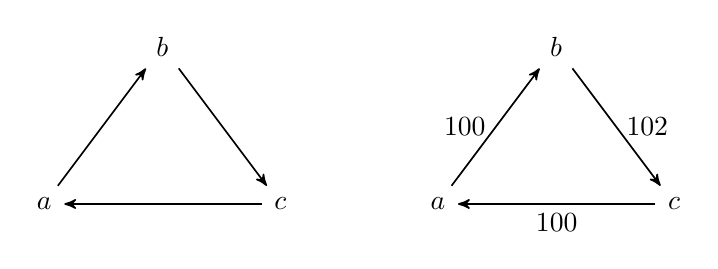
\begin{tikzpicture}[->,>=stealth',shorten >=1pt,shorten <=1pt, auto,node distance=1.5cm,semithick]
        \node (a) at (0,0) {$a$};
        \node (b) at (1.5,2) {$b$};
        \node (c) at (3,0) {$c$};
        \node (a') at (5,0) {$a$};
        \node (b') at (6.5,2) {$b$};
        \node (c') at (8,0) {$c$};

        \path[->] (a) edge (b);
        \path[->] (b) edge (c);
        \path[->] (c) edge (a);
        \path[->] (a') edge node[left]{100} (b');
        \path[->] (b') edge node[right]{102} (c');
        \path[->] (c') edge node[below]{100} (a');
    \end{tikzpicture}
\end{center}

The next voting rule use \textit{Copeland scores} to select winners. A (symmetric) Copeland score of alternative $x$ is:
\begin{definition}[(symmetric) Copeland score]
    $\mathit{Copeland}(x) = |\{y \in A\;|\; x >^\mu y\}| - |\{y \in A\;|\; y >^\mu x\}|$
\end{definition}

The Copeland rule selects the alternative(s) with highest Copeland score. In $\profile_1$ for example, $a$'s Copeland scores is $0$, since $a \pma b$ and $c \pma a$. So as $b \mbox{ and } c$. Thus the winning set of $\profile_1$ is $\{a,b,c\}$.

\subsection{Borda}

In the case of Copeland rule, for every alternative $a$, all we care about is how many times $a$ has been defeated and won. However, as we can notice, the margins of victory or defeat matter as well. If we take these margins into consideration, things will be different.

Given a profile $\profile$, the \textit{symmetric Borda score} of an alternative $x$ is\footnote{Noted that the definition here is nonstandard, the standard version will come up later.}:
\begin{definition}[symmetric Borda score]
    \label{sbor}
    $\mathit{Borda}^{\mathit{sym}}_\profile (x) = \sum_{y \in A} \mathit{Net}_\profile (x > y)$
\end{definition}

Under Borda rule, alternative(s) with the highest Borda score is the winner(s). In $\profile_1$, the scores of $a,b,c$ are $0,2,-2$ respectively, thus the winner is $b$.

A more common asymmetric Borda score is defined via the \textit{vector of scoring weights} (score vector) $\mathbf{w}$:

\begin{definition}[asymmetric Borda score]
    For $|A| = m$. Let $\mathbf{w} = {m-1,m-2,m-3,\dots,0}$. $\mathit{Borda}^{\mathit{asym}}_\profile (x)$ is the sum of points awarded to x by all voters, where for voter $i$, if $a$ is top-ranked then $a$ get $(m-1)$ points, if the next then $(m-2)$\dots\dots, and $0$ to the least preferred.
\end{definition}

Noted that the two versions of Borda score are affinely equivalent, with $\mathit{Borda}^{\mathit{asym}}_\profile (x) = n + \frac{1}{2} \mathit{Borda}^{\mathit{sym}}_\profile (x)$, so they induce the same SCF\footnote{Don't understand what `affinely' mean\dots\dots}. Actually, if we make $\mathbf{w} = \{m-1,m-3,m-5,\dots,-(m-1)\}$, then we replicate the scores from \cref{sbor}. An adventage of symmetric approach is that it's well-defined for profiles which is weak preferences, thus the symmetric Copeland and Borda rules can be extended to weak preference cases.

\subsection{Social Choice Function}

Let $\mathcal{C}(X)$ denote the set of all nonempty subsets of a set $X$.

\begin{definition}[social choice function]
    \label{SCF}
    \begin{itemize}
        \item A \textit{social choice function} (SCF) is a map $f:\; \linearor^n \to \ca$ that returns a nonempty set of alternatives for each profile of strict preference.
        \item If $f(\profile) = 1$ then $f$ is \textit{single valued} on $\profile$ and sometimes we write $f(\profile) = x$ instead of $f(\profile) = \{x\}$.
        \item A \textit{resolute} SCF is one with no tied: it's single valued on all profiles.
    \end{itemize}
\end{definition}

Above are fixed electorate SCFs. We can substitude $\linearor^\infty$ for $\linearor^n$, from which we get variable electorate SCFs. Notice that the rest of this chapter presumes a fixed electorate, except where explicitly noted otherwise.

In \cref{SCF}, the value of the function is a group of winners, while in preceding three rules, we not only concentrate on the winner(s), but also the "social ranking"---one alternative is ranked over another if it has a higher score. Here we don't restrict the ranking to be strict, which leads to the definition below:

\begin{definition}[social welfare function]
    A \textit{social welfare function} (SWF), is a map $f:\; \linearor^n \to \weakor$ that returns a weak ranking of the set of alternatives for each profile of strict preferences.
\end{definition}

\subsection{Strategic Manipulation}

Now we take a look at some occasions where voters may have an incentive to cast insincere ballots under such voting rules.

Consider Ali, one of the two $a \succ b \succ c \succ d \succ e$ voters of profile $\profile_2$.
\begin{center}
    \begin{tabular}{ccc}
        2 & 3 & 2\\
        \hline
        $e$ & $ d $ & $ a$\\
        $c $&$ e $&$ b$\\
        $a $&$ b $&$ c$\\
        $d $&$ c $&$ d$\\
        $b $&$ a $&$ e$
    \end{tabular}
\end{center}

Under Copeland, Ali's least preferred alternative $e$ wins: $e$'s (symmetric) Copeland score is $2$, $b$'s is $-2$ and the other scores are each $0$. However, if Ali misrepresents his sincere preferences as a reverse of his ranking, the Copeland winner shifts to $d$, where $d \succ_{Ali} e$, with a score of $4$, the maximum possible.

\begin{definition}
    \begin{itemize}
        \item An SCF $f$ is \textit{single voter manipulable} if for some pair $\profile,\, \profile'$ of profiles on which $f$ is single valued, and voter $i$ with $\succsim'_j = \succsim_j$ for all $j \neq i$, $f(\profile') \succ_i f(\profile)$;
        \item $f$ is \textit{single voter strategyproof} if it's not single voter manipulable.
    \end{itemize}
\end{definition}

$\succ_i$ stands for the sincere preference, while $\succ'_i$ is the insincere one. An SCF being single voter manipulable means that if voters give an insincere ranking then he'll get a better result.

Under Copeland rule, Ali has to reverse the ballot. And under Borda rule, he can still do such things---by just lifting $d$ to the top position ($d \succ a \succ b \succ c \succ e$).

Plurality voting is not single voter manipulable, since it only care about the top-ranked alternatives. Any voter who wants $x$ rather than $y$ to be the winner won't place $y$ in the top on his sincere ballot, so he cannot lower $y$'s score. But if there's two voters switching there ballot, then Plurality voting can be manipulable as well.

Obviously voting rules with ties or single voter manipulable is inappropriate, thus we have to deal with such problem. That's what we do in the later section.
\section{Axioms I: Anonymity, Neutrality, and the Pareto Property}

From now on, we switch to the \textit{axiomatic method} to identify voting rules. Axioms of SCFs can be loosely divided into three groups:
\begin{itemize}
    \item \textit{the First Group:} Axioms here represent the minimal demands, which has been seen as uncontroversial;
    \item \textit{the Second Group (or Middling Strength):} They are satisfied by some interesting SCFs, but the cost is high, since it rules out many attractive voting rules;
    \item \textit{the Third Group:} They are the strongest, including IIA and strategyproofness, in that they tend to rule out all reasonable voting rules.
\end{itemize}

In this section we mainly discuss five axioms from the first group. Let $f$ be an SCF.

\begin{definition}
    \begin{itemize}
        \item \textbf{Anonymous:} $f$ is anonymous if each pair of voters plays interchangeable roles: $f(\profile) = f(\profile^\star)$ holds if for $i, j \in N$, $\succsim^\star_i = \succsim_j,\; \succsim^\star_j = \succsim_i$, and $\succsim^\star_k = \succsim_k$ for all $k \neq i,j$.
        \item \textbf{Dictatorial:} $f$ is dictatorial if for some $i \in N$, $i$ act as dictator, i.e. for all profile $\profile$ and $a \in A$, if $a \succ_i b$ holds for all $b \in A$, then $f(\profile) = a$.
        \item \textbf{Neutral: } $f$ is neutral if each pair of alternatives are interchangeable in the following sence: whenever a profile $\profile^\dagger$ is obtained from another $\profile$ by swapping the positions of the two alternatives $x$ and $y$ in every ballot, the outcome $f(\profile^\dagger)$ is obtained from $f(\profile)$ via a similar swap.
        \item \textbf{Imposed:} $f$ is imposed if for no profile $\profile$ does $f(\profile) = \{x\}$.
        \item Given a profile $\profile$ and $x,y \in A$, we say that $x$ \textit{Pareto dominates} $y$ if every voter ranks $x$ over $y$; and $y$ is called being Pareto dominated if such an $x$ exists.
        \item \textbf{Pareto Principle:} $f$ is Pareto (Pareto optimal, or Paretian) if $f(\profile)$ never contains a Pareto dominated alternative.
    \end{itemize}
\end{definition}

Noted that \textit{anonymity} and \textit{neutrality} are strong forms of equal treatment of voters, \textit{nondictatoriality} serves as a particularly weak version of anonymous, and \textit{nonimposition} serves as a particularly weak version of neutrality. We also have Pareto implies nonimposition.

The voting rules mentioned above (Plurality, Copeland and Borda) are anonymous, neutral and Pareto, while reverse Borda\footnote{“Reverse Borda” SCF: elect the alternative(s) having the lowest Borda score.} is not Pareto. Although being uncontroversial, these three axioms do leads to unintended consequences, which is mentioned in \cite{moulin2014strategy}. 

\begin{proposition}
    \label{nonresolute}
    Let $m \geq 2$ be the number of alternatives and $n$ be the number of voters. If $n$ is divisible by any integer $r$ with $1 < r \leq m$, then no neutral, anonymous and Pareto SCF is resolute (single-valued).
\end{proposition}

\begin{proof}
    For $m \geq 3$ (with $A = \{a,b,c,x_1,\dots,x_{m-3}\}$) and $n = 3k$. Consider a profile $\profile$ as following.
    \begin{center}
        \begin{tabular}{ccc}
            $k$ & $k$ & $k$\\
            \hline
            $a$ & $c$ & $b$\\
            $b$ & $a$ & $c$\\
            $c$ & $b$ & $a$\\
            $x_1$ & $x_1$ & $x_1$\\
            $\vdots$ & $\vdots$ & $\vdots$
        \end{tabular}
    \end{center}
    We show that $f(\profile) = \{a,b,c\}$.
    Since $f$ is Pareto, $f(\profile) \subseteq \{a,b,c\}$. W.l.o.g. $a \in f(\profile)$. First we swap the position of $a$ and $b$, then $b$ and $c$, finally we'll get a profile $\profile'$ which remains the same as $\profile$. Thus we have $c \in f(\profile)$ since $f$ is neutral. Analogously we can prove that $b \in f(\profile)$. \\
    Using the same method we can extend the conclusion above to the case in \cref{nonresolute}.
\end{proof}

\cref{nonresolute} tell us that we have to deal with ties in the outcome. In \cite{brandt_handbook_2016} he come up with four method trying to solve the problem:

\begin{enumerate}
    \item Use a fixed ordering of the alternatives (or a designated voter) to break all ties.
    \item Use a randomized mechanism to break all ties.
    \item Deal with set-valued outcomes directly.
    \item Ignore or suppress the issue (assume no ties exist).
\end{enumerate}

\section{Voting Rules I: Condorcet Extensions, Scoring Rules, and Run-Offs}

Introduce two axioms here:\\

\begin{definition}
    \begin{itemize}
        \item \textit{monotonicity}: if $x$ is the winner and one voter switches his ballot from $y$ to $x$, then $x$ is still a winner; 
        \item \textit{positive responsiveness}: if $x$ is a winner and one voter switches her ballot from $y$ to $x$, then $x$ becomes the unique winner.
    \end{itemize}
\end{definition}

Now we concentrate on the \textit{Majority rule}, which suits for the case when the number of alternatives is $2$. Majority rule, which selects the alternative with more votes as winner, is anonymous, neutral and resolute when the number of voters is odd. In additional, the characterizition of it requires \textit{monotonicity} or \textit{positive responsiveness}.

\begin{proposition}[May's Theorem]
    \label{ThMay}
    For two alternatives and an odd number of voters, majority rule is the unique resolute, anonymous, neutral, and monotonic SCF. For two alternatives and any number of voters, it is the unique anonymous, neutral, and positively responsive SCF.
\end{proposition}

\begin{proof}
    Obviously majority rule satisfies these properties. For uniqueness, consider any other rules that selects the alternative with fewer votes as the winner. Let $A = \{a,b\}$ and $N = \{1,\dots,n\}$ with $n$ being odd. W.l.o.g. $|\{i \in N\;|\; a \succ_i b\}| = k_1$ and $|\{j \in N\;|\; b \succ_j a\}| = k_2$ where $k_1 + k_2 = n$ and $k_1 < k_2$. According to the rule, $a$ is the winner. Then we switch enough ballots to form a new profile where $|\{i \in N\;|\; a \succ_i b\}| = k_2$ and $|\{j \in N\;|\; b \succ_j a\}| = k_1$. $b$ will be the winner by neutrality, while monotonicity implies $a$ is still the winner, from which we get a contradiction. Analogously we can prove the other case.
\end{proof}

\cref{ThMay} tells us that majority rule is the best voting rule when $|A| = 2$. Since all other SCFs considered so far can be reduced to majority rule in the case of two alternatives, we can also say that these SCFs can be seen as "majority rule for 3 of more alternatives". But for SCFs with a full domain ($\mathrm{Dom}(f) = \linearor^{<\infty}$), there is no complitely satisfactory extension of May's Theorem to the case of $|A| \geq 3$.

There's another rule which is considered deserving:

\begin{definition}[Condorcet winner]
    A \textit{Condorcet winner} for a profile $\profile$ is an alternative $x$ that defeats every other alternative in the strict pairwise majority sense: $x >^\mu_\profile y$ for all $y \neq x$\footnote{The weak version is $x \geq^\mu_\profile y$ for all $y \neq x$}.\\
    \textit{Pairwise Majority Rule (PMR)} declares the winning alternative to be the Condorcet winner, and is undefined when a profile has no Condorcet winner.
\end{definition}

Whenever a Condorcet winner exists, it must be unique. But with $|A| \geq 3$, it might forms \textit{majority cycles} which rule them out, then no PMR winner exists. The majority cycle is known as \textit{Condorcet's voting paradox}, which reminds us that $>^\mu$ is intranstive.

Notice that PMR is an SCF with \textit{restricted domain}, since it has the possibility that no winner exists. Our interest here is with full SCFs that agree with PMR on its domain:

\begin{definition}
    \begin{itemize}
        \item \textit{Condorcet domain:} $\condom = \{\profile\;|\; \profile \mbox{ has a Condorcet winner}\}$;
        \item An SCF $f$ is \textit{Condorcet extension (consistent):} if for all $\profile \in \condom$, $f$ selects the Condorcet winner alone.
    \end{itemize}
\end{definition}

\begin{proposition}[Campbell-Kelly Theorem]
    \label{ThCK}
    Consider SCFs with domain $\condom$ for three or more alternatives. Pairwise Majority Rule is resolute, anonymous, neutral, and strategyproof; for an odd number of voters, it is the unique such rule.
\end{proposition}

If we restrict $f$'s domain to $\condom$, then \cref{ThCK} can be seen as “May's Theorem for three or more alternatives”, specially for strategyproof, when $|A| = 2$ it can be shown that monotonicity is equivalent to strategyproof.

\begin{proof}
    Clearly, restricted to $\condom$, PMR is resolute, anonymous and neutral. For strategyproof, conside a voter $i$ with the sincere ballot being $y \succ_i x$ for alternatives $x,y$, and the Condorcet winner is $x$. Then however $i$ changes his ballot, $x$ remains to be the winner.\\
    For uniqueness\dots
\end{proof}

Note that Condorcet extension isn't necessary when choosing a voting rule. Borda is not a Condorcet extension actually, consider a profile $\profile$ with $|N| = 5$ and $A = \{a,b,c\}$, if three voters rank $a \succ b \succ c$ and two rank $b \succ c \succ a$\dots. And Copeland rule is a Condorcet extension.

Condorcet extensions form the first class of voting rules. The second class is \textit{scoring rules}:

\begin{definition}
    \begin{itemize}
        \item A \textit{score vector} $\mathbf{w} = (w_1,w_2,\dots,w_m)$ consists of real number \textit{scoring weights}. 
        \item $\mathbf{w}$ is \textit{proper} if $w_1 \geq w_2 \geq \dots \geq w_m$ and $w_1 > w_m$.
        \item A \textit{proper scoring rule} is one induced by a proper score vector, in which each voter awards $w_1$ points to their top-ranked alternative, $w_2$ points to their second-ranked, and so on. All points awarded to a given alternative are summed, and the winner is the alternative(s) with greatest sum.
    \end{itemize}
\end{definition}

\label{run-off}
The third class consists \textit{multiround rules}, which is based on the idea that less popular alternatives in one round be dropped from all ballots in the next round (with each ballot then ranking the remaining alternatives in the same relative order that they had in the initial version of that ballot); these rounds continue until some surviving alternative achieves majority support (or until only one is left standing).

\section{An Informational Basis for Voting Rules: Fishburn's Classification}

Fishburn divided SCFs into three classes according to the information required in them:
\begin{itemize}
    \item \textit{C1 functions}: SCFs which need only the information from the tournament;
    \item \textit{C2 functions}: SCFs which need the additional information in the weighted tournament;
    \item \textit{C3 functions}: SCFs which are neither C1 nor C2, plurality for example.
\end{itemize}
\section{Axioms II: Reinforcement and Monotonicity Properties}

In this part, we mainly discuss the second group of the axioms, which are about profile changes when adding more voters or changing several voters' ballots. Hence we need variable electorate context and voting situation: for $s,t:\; \linearor \to \mathbb{Z}^+$\footnote{$s,t$ can be regarded as two group of voters with different ballots.}. For simplicity, we fix the following conventions:
\begin{itemize}
    \item $s+t$ stands for putting $s$ and $t$ together in one voter-set;
    \item $ks\;(k \in \mathbb{N})$ stands for replacing each individual voter of s with k “clones”.
\end{itemize}

\begin{definition}[Reinforcement (aka Consistency)]
    An SCF $f$ is reinforcing if $f(s) \cap f(t) \neq \emptyset \Rightarrow f(s+t) = f(s) \cap f(t)$.
\end{definition}

Intuitively, reinforcement requires that the common winning alternatives chosen by two disjoint sets of voters (if there exists) be exactly those chosen by the union of these sets. Specially if $f(s) = f(t)$ then $f(s+t) = f(s) = f(t)$.

There's also a weak form of reinforcement:
\begin{definition}[Homogeneity]
    $f(ks) = f(s)$ for all $k \in \N$.
\end{definition}

Noted that all scoring rules are reinforcing, since if some alternatives get the highest score both in $s$ and $t$, then they must have the highest score in $s+t$. Analogously we can apply the same argument to \textit{compound scoring rules}.

\begin{definition}[Compound Scoring Rules]
    A voting rule is a \textit{compound scoring rule} if any ties resulting from a first score vector $\mathbf{w}_1$ may be broken by score differences arising from a second such vector $\mathbf{w_2}$, with a possible third vector used to break ties that still remain, and so on; any finite number $j \geq 1$ of score vectors may be used.\\
    A \textit{simple scoring rule} is the scoring rule which is not compound.
\end{definition}

Notice that on a domain that is restricted by fixing an upper bound on the number of voters, every such compound rule is equivalent to some simple scoring rule\footnote{Why??????Anyone can tell me why\dots?????????}.

\begin{theorem}[See \textcite{John_compound} and \textcite{young_social_1975}]
    The anonymous, neutral, and reinforcing SCFs are exactly the compound scoring rules.
\end{theorem}

\begin{proof}
    886
\end{proof}

\begin{proposition}
    All Condorcet extension SCFs for three or more alternatives violate reinforcement.
\end{proposition}

\begin{proof}
    Consider voting situation $s$ and $t$ with 3 alternatives below:\\
    ~\\
    \begin{minipage}{0.5\textwidth}
        \begin{center}
            \begin{tabular}{ccc}
                2 & 2 & 2\\
                \hline
                a & c & b\\
                b & a & c\\
                c & b & a
            \end{tabular}
        \end{center}
    \end{minipage}
    \begin{minipage}{0.4\textwidth}
            \begin{tabular}{cc}
                2 & 1\\
                \hline
                b & a \\
                a & b\\
                c & c
            \end{tabular}
    \end{minipage}
    \\
    Let $f$ be any Condorcet extension. Since $b$ is the Condorcet winner in $t$, we have $f(t) = \{b\}$. Also $a$ is the Condorcet winner in $(s+t)$, thus $f(s+t) = \{a\}$. If $f$ is reinforcing then $a \in f(t)$ should hold, which leads to a contradiction.\\
    If we assume $f$ to be Pareto, then it's easy to extend our construction to a general form, just by adding other alternatives $x_i$ behind $a,b,c$ in the voting situation. If not, we have to find another more complicated voting situation as a counterexample.
\end{proof}

\noindent Intuitively, for a winner $a$, if we move $a$ from under some alternatives to over them in some voters' preference, without changing the relative order of other pair of alternatives excluded $a$, then $a$ still should be the winner (\textit{simple lift}). That's what \textit{monotonicity} said.

\begin{definition}
    A resolute SCF $f$ satisfies \textit{monotonicity} (aka weak monotonicity) if whenever a profile $\profile$ is modified to $\profile'$ by having one voter $i$ switch $\succsim_i$ to $\succsim'_i$ by lifting the winning alternative $x = f(\profile)$ simply, $f(\profile') = f(\profile)$.
\end{definition}

Notice that here we require that $f(\profile)$ is single-valued, if not, then the definition only cares about the cases when $|f(\profile)| = 1$.

Suppose $f$ is a voting rule which select the alternative(s) with highest score, and lifting alternatives $x$ never lower $x$'s score or raise $y$'s score for $ y \neq x$. Then $f$ is always monotonic. It follows that all proper scoring rules are monotonic.
However, each of scoring run-off rule is not monotonic\footnote{For scoring run-off rules, see the last part of \cref{run-off}.}. I omitted the proof here since it seems to do with some knowledge of computation\dots

\begin{remark}
    Every resolute SCF $f$ which violate monotonicity implies that there's an opportunity for voter $i$ manipulate $f$ by simple lifting or dropping an alternative:\\
    Let $\succ_i \mapsto \succ'_i$ by a simple lift of he winning alternative $a$ which makes $b$ win and $a$ lose. If $b \succ_i a$, then the voter with sincere ballot $\succ_i$ would gain by casting the insincere ballot $\succ'_i$ and vice versa.
\end{remark}

Thus monotonicity is a weak form of strategyproofness. Below are some relavent definitions:

\begin{definition}
    A resolute SCF $f$ satisfies:
    \begin{itemize}
        \item \textit{Strategyproofness} if whenever a profile $\profile$ is modified to $\profile'$ by having one voter $i$ switch $\succsim_i$ to $\succsim'_i$ , $f(\profile) \succsim_i f(\profile')$.
        \item \textit{Maskin monotonicity} (aka \textit{strong monotonicity}) if whenever a profile $\profile$ is modified to $\profile'$ by having one voter $i$ switch $\succsim_i$ to a ballot $\succsim'_i$ satisfying for all $y,\; f(\profile) \succsim_i y \Rightarrow f(\profile) \succsim'_i y$ then $f(\profile') = f(\profile)$\footnote{See \textcite{maskin1999}. The original definition is based on not only resolute SCF: $f$ is Maskin monotonic if $\forall a \in f(\profile)$, if $\forall i \in N,\; \forall b \in A,\; a \succsim_i b \Rightarrow a \succsim'_i b$, then $a \in f(\profile')$. It can be understood as, if $a$ does not fall below any alternatives that it was not below before, then $a$ will still be the winner.}.
        \item \textit{Down monotonicity} if whenever a profile $\profile$ is modified to $\profile'$ by having one voter $i$ switch $\succsim_i$ to $\succsim'_i$ by dropping a losing alternative $b \neq f(\profile)$ simply, $f(\profile') = f(\profile)$.
        \item \textit{One-way monotonicity} if whenever a profile $\profile$ is modified to $\profile'$ by having one voter $i$ switch $\succsim_i$ to $\succsim'_i$, $f(\profile) \succsim_i f(\profile')$ or $f(\profile') \succsim_i f(\profile)$\footnote{See \textcite{sanver_one-way_2009}: It asserts that whenever one identification represents a successful manipulation, the other represents a failure.}
        \item \textit{Half-way monotonicity} if whenever a profile $\profile$ is modified to $\profile'$ by having one voter $i$ switch $\succsim_i$ to $\succsim^{rev}_i$, $f(\profile) \succsim_i f(\profile')$, where $\succsim^{rev}$ denotes the reverse of $\succsim$.
        \item \textit{Participation} (the absence of no show paradoxes) if whenever a profile $\profile$ is modified to $\profile'$ by adding one voter $i$ with ballot $\succsim_i$ to the electorate, $f(\profile') \succsim_i f(\profile)$.
    \end{itemize}
\end{definition}

Participation is a corresponding version of strategyproofness for no-show paradox. No-show paradox, first come up by \textcite{fishburn_paradoxes_1983}, also mentioned by \textcite{sanver_one-way_2009}, shows that, one additional participating voter shows up to cast her vote, and the winner is then an alternative that is strictly inferior (according to the preferences of the participating voter) to the alternative who would have won had she not shown up. Thus the paradox implies an opportunity to manipulate by abstaining.

\begin{proposition}
    For resolute SCFs:
    \begin{enumerate}
        \item Strategyproofness $\Rightarrow$ Maskin monotonicity $\Leftrightarrow$ Down monotonicity $\Rightarrow$ monotonicity
        \item Strategyproofness $\Rightarrow$ One-way monotonicity $\Rightarrow$ Half-way monotonicity
        \item Participation $\Rightarrow$ monotonicity
    \end{enumerate}
\end{proposition}

\begin{proof}
    The proof of \textit{Item I} and \textit{Item II} is straightforward, except for the first arrow in Item I. Consider an SCF $f$ which violates Maskin monotonicity. Let $a, b \in A$, $\profile$ be a profile where $f(\profile) = \{a\}$ and for voter $i$, $b \succsim_i a$. Now $\profile'$ is modified from $\profile$ by changing $b \succsim_i a$ to $a \succsim_i b$, and $f(\profile') \neq \{a\}$. 
    If $f(\profile') = \{b\}$ or any other alternatives $c$ with $c \succsim_i a$, then a voter with sincere preference $\succsim_i$ would gain a better result by casting the insincere ballot $\succsim'_i$. Otherwise a voter with sincere preference $\succsim'_i$ can change his ballot to $\succsim$. Thus $f$ is not strategyproofness.\\
    For \textit{Item III}, see \textcite{sanver_one-way_2009}. Note that the original proof aims at proving participation $\Rightarrow$ one-way monotonicity,  but failed.\\
    Let $\profile \in \mathrm{Dom}(f)$ be a profile and $s,t$ be two preference given by two voters $s \mbox{ and } t$ seperately. Assume that $f$ is an SCF satisfying participation with $f(\profile \wedge s) = a$ and $f(\profile \wedge t) = b$, we show that $a \succsim_s b$ or $b \succsim_t a$. Consider 3 cases:
    \begin{itemize}
        \item \textit{Case 1:} $f(\profile) = a$ or $f(\profile) = b$. If $f(\profile) = a$, since $f(\profile \wedge t) = b$, $b \succsim_t a$ by participation; if $f(\profile) = b$, then similarly $a \succsim_s b$.
        \item \textit{Case 2:} $f(\profile \wedge s \wedge t) = a$ or $f(\profile \wedge s \wedge t) = b$. It's analogous to the preceding case.
        \item \textit{Case 3:} $f(\profile) = x$ with $x \not \in \{s,t\}$ and $f(\profile \wedge s \wedge t) = y$ with $y \not \in \{s,t\}$. By participation we have $a \succsim_s x$, $b \succsim_t x$, $y \succsim_s b$ and $y \succsim_t a$. If $\succsim_s = \succsim^{rev}_t$ then $a \succsim_s x$ and $x \succsim_s b$, thus $a \succsim_s b$ as desired.
    \end{itemize}
\end{proof}
\section{Strategyproofness: Impossibilities}\label{straproof_imp}

In this section, we go into Gibbard-Satterthwaite Theorem, which claims that Any resolute, nonimposed, and strategyproof SCF for three or more alternatives must be a dictatorship. Conversely, we can find that every resolute, nonimposed, and nondictatorial SCF for three or more alternatives is manipulable.

\begin{theorem}[Gibbard-Satterthwaite Theorem]
    \label{GSTheorem}
    Any resolute, nonimposed, and strategyproof SCF for three or more alternatives must be a dictatorship.
\end{theorem}

Begin with the following definition:

\begin{definition}
    Let $f$ be a resolute social choice function for $m \geq 3$ alternatives, $a, b \in A$ be two distinct alternatives and $X \subseteq N$ be a set of voters. Then we say that $X$ can use $a$ to block $b$, notated $X_{a > b}$, if for every profile $\profile$ wherein each voter in $X$ ranks $a$ over $b$, $f(\profile) \neq b$; \\
    $X$ is a \emph{dictating set} if $X_{z>w}$ holds for every choice $z \neq w$ of distinct alternatives.
\end{definition}

\begin{lemma}[Push-Down Lemma]
    \label{push_down_lemma}
    Let $a,b,c_1,c_2,\dots,c_{m-2}$ enumerate the $m \geq 3$ alternatives in $A$, $f$ be a resolute and down monotonic SCF for $A$, and $\profile$ be any profile with $f(\profile) = a$. Then there exists a profile $\profile^\star$ with $f (\profile^\star) = a$ such that:
    \begin{itemize}
        \item For every voter $i$ with $a \succ_i b$: $\succ^\star_i = a \succ b \succ c_1 \succ \dots \succ c_{m-2}$;
        \item For every voter $i$ with $b \succ_i a$: $\succ^\star_i = b \succ a \succ c_1 \succ \dots \succ c_{m-2}$;
    \end{itemize}
\end{lemma}

\begin{proof}
    The proof is quite intuitive, due to $f$ being down monotonic, $\profile^\star$ can be formed just by dropping simply $c_1,\dots,c_{m-2}$ to the bottom of each ranking one by one. 
\end{proof}

\begin{lemma}
    \label{block_set}
    Let $f$ be a resolute and down monotonic SCF. If there exists a profile $\profile$ for which every voter in $X$ has $a$ over $b$, every voter in $N \backslash X$ has $b$ over $a$, and $f (\profile) = a$, then $X_{a>b}$.
\end{lemma}

\begin{proof}
    Suppose (towards a contradiction) that there is a $\profile$ as stated and not $X_{a>b}$. Choose a second profile $\profile'$ s.t. each voter in $X$ rank $a$ above $b$ and $f(\profile') = b$. If any $\profile'$ voters in $N \backslash X$ have $a$ over $b$, then let them one-at-a-time drop $a$ simply below $b$ to get another new profile $\profile''$. Due to $f$ being down monotonic, $f(\profile'') = b$.
    Applying \cref{push_down_lemma} to both $\profile$ and $\profile''$, we get $\profile^\star$ with $f(\profile^\star) = a$ and $\profile''^\star$ with $f(\profile''^\star) = b$. However, $\profile^\star = \profile''^\star$, contradict.
\end{proof}

\begin{lemma}
    \label{disjoint_sets}
    Let $f$ be a resolute, Pareto, and down monotonic SCF for three or more alternatives. Assume $X_{a>b}$, with $X = Y \cup Z$ split into disjoint subsets $Y$ and $Z$. Let $c$ be any alternative distinct from $a$ and $b$. Then $Y_{a>c}$ or $Z_{c>b}$.
\end{lemma}

\begin{proof}
    Consider a profile below:
    $$
    \begin{array}{ccc}
        Y & Z & N \backslash X\\
        \hline
        a & c & b\\
        b & a & c\\
        c & b & a\\
        \vdots & \vdots & \vdots
    \end{array}
    $$
    Since $f$ is Pareto, $f(\profile) \in \{a,b,c\}$. According to the assumption that $X_{a>b}$, $f(\profile) \neq b$. If $f(\profile) = a$, then by \cref{block_set}, $Y_{a>c}$. Otherwise, $Z_{c>b}$.
\end{proof}

\begin{lemma}
    \label{X_itself}
    Let $f$ be a resolute, Pareto, and down monotonic SCF for three or more alternatives. Assume $X_{a>b}$.Let $c$ be any alternative distinct from $a$ and $b$. Then (i) $X_{a>c}$ and (ii) $X_{c>b}$.
\end{lemma}

\begin{proof}
    Noted that none of conditions in \cref{disjoint_sets} rules out the possibilities of $Y$ or $Z$ being empty. And Pareto implies that $\emptyset_{z>w}$ is impossible. Thus let $X = Y$ and $Z = \emptyset$ in last proof, then we have $X_{a>c}$. Analogously let $Y = \emptyset$, then $X_{c>b}$.
\end{proof}

\begin{lemma}
    \label{dictating_set}
    Let $f$ be a resolute, Pareto, and down monotonic SCF for three or more alternatives. Assume $X_{a>b}$. Then $X$ is a dictating set.
\end{lemma}

\begin{proof}
    Let $a,b,y\in A$ and $X_{a>b}$ hold. We show that $X_{y>z}$ holds for every $z \neq y$. Consider several cases below:
    \begin{itemize}
        \item[\textit{Case 1:}] $y = a$. By \cref{X_itself} (i), we already have for all $z$ distinct from $a$, $X_{a>z}$.
        \item[\textit{Case 2:}] $y \not \in \{a,b\}$. By \cref{X_itself}, $X_{y>b}$. Applying \cref{X_itself} to $X_{y>b}$ again, we then have for every $z$ dsitinct from $y$ and $b$, $X_{y>z}$.
        \item[\textit{Case 3:}] $y = b$. First $X_{a>c}$ holds for $c$ distinct from $a$ and $y$. Then $X_{y>c}$ since $y$ is distinct from $a$ and $c$. Finally we get $X_{y>z}$ from all $z \neq b$.
    \end{itemize}
\end{proof}

\begin{lemma}[Splitting Lemma]
    \label{splitting_lemma}
    Let $f$ be a resolute, Pareto, and down monotonic SCF for three or more alternatives. If a dictating set $X = Y \cup Z$ is split into disjoint subsets $Y$ and $Z$, then either $Y$ is a dictating set, or $Z$ is.
\end{lemma}

\begin{proof}
    Since $X_{a>b}$, by \cref{disjoint_sets}, either $Y_{a>c}$ or $Z_{c>b}$. Using \cref{dictating_set}, either $Y$ is a dictating set of $Z$ is.
\end{proof}

\begin{lemma}[Adjustment Lemma]
    \label{Adjustment_lemma}
    Let $f$ be any resolute, nonimposed SCF (but no longer assume $f$ is Pareto). If $f$ is down monotonic then it is Pareto.
\end{lemma}

\begin{proof}
    Suppose ($\lightning$) that $f$ is not Pareto, i.e. there is a profile $\profile$ s.t. every voter ranks $b$ over $a$ while $f(\profile) = a$. Choose a second profile $\profile'$ with $f(\profile') = b$. Due to $f$ being nonimposed, such a profile nust exist. Now if any voter in $\profile'$ ranks $a$ over $b$, then let him one-at-a-time drop $a$ simply below $b$. By down monotonicity, the resulting profile $\profile''$ satisfies $f(\profile'') = b$. Applying \cref{push_down_lemma} to $\profile$ and $\profile''$ to obtain $\profile^\star$ and $\profile''^\star$ with $\profile^\star = \profile''^\star$, while $f(\profile^\star) = a$ and $f(\profile''^\star) = b$
\end{proof}

\begin{proof}[for Gibbard-Satterthwaite Theorem]
    ~\\
    Let $f$ be an SCF satisfying resolute, nonimposed, and strategyproof. Recall \cref{monotonicitys}, $f$ is down monotonic as well. Applying \cref{Adjustment_lemma} we know $f$ is Pareto, thus $N$ itself is a dictating set. Using \cref{splitting_lemma} repeatedly until a singleton has been left, then by \cref{X_itself} and \cref{dictating_set} the singleton is a dictating set.
\end{proof}

There is also a well known variant reformulating \cref{GSTheorem} in terms of monotonicity.

\begin{theorem}
    Any resolute, nonimposed, and Maskin monotonic SCF for three or more alternatives must be a dictatorship.
\end{theorem}

The proof is easy, since Maskin monotonicity implies down monotonicity (\cref{monotonicitys}).\\
~\\
Gibbard-Satterthwaite Theorem seems to give us a negative result, indicating that many voting rules are manipulable. Nevertheless, we should also note that there are manifold limitations inside it.

\begin{enumerate}
    \item It's nearly impossible to achieve a fulfillment of all conditions for single voter manipulation, since if one want to manipulate, at least she has to have access to other's ballot and make sure anyone except her won't manipulate.
    \item The theorem applies only to the social choice function context, with its associated form of ballot---ordinal rankings of the alternatives---and of election outcome. For example, \textit{Social Decision Schemes} escape the Gibbard-Satterthwaite context at the other end---the output---by declaring a probability distribution as the election outcome.
    \item The theorem only applied to \emph{resolute} SCFs. However, in \cref{nonresolute} we have known, in the case of a neutral and anonymous SCF $f$ , ties are often inevitable, suggesting that the theorem might say little about the rules that are of greatest interest.
\end{enumerate}

Now we turn to another significant question, asking that \emph{How many tied outcomes must we be willing to live with, in order to achieve strategyproofness?} Several generalizations of Gibbard-Satterthwaite to irresolute SCFs suggest an answer: \emph{a lot of ties}. To prove it, we first fix some conventions:

\begin{definition}
    \begin{itemize}
        \item For $Z \subseteq A$, let $\mbox{max}_{\succ_i}[Z]$ denote $i$'s top ranked alternative in $Z$ and $\mbox{min}_{succ_i}[Z]$ similarly.
        \item Let $f$ be an SCF, possibly irresolute. We say $f$ is \emph{manipulable by optimists} if for some pair $\profile,\profile'$ of profiles and voter $i$ with $\succsim'_j = succsim_j$ for all $j \neq i$, $\mbox{max}_{\succ_i} [f(\profile')] \; \succ_i \; \mbox{max}_{\succ_i} [f(\profile)]$.
        \item $f$ is \emph{manipulable by pessimists} if for some pair $\profile,\profile'$ of profiles and voter $i$ with $\succsim'_j = \succsim_j$ for all $j \neq i$, $\mbox{min}_{\succ_i} [f(\profile')] \; \succ_i \; \mbox{min}_{\succ_i} [f(\profile)]$.
        \item A voter $k$ is a nominator for $f$ if for every profile $\profile$, $k$'s top-ranked alternative is a member of $f(\profile)$.
        \item The \emph{Omninominator} SCF returns, for each profile $\profile$, the set $\textit{OmNom}(\profile)$ of all alternatives that have been top-ranked by at least one voter.
    \end{itemize}
\end{definition}

The intuition here is that some outside agency will ultimately choose a single winning alternative from the set $f(\profile)$. An ``optimist'' assumes that the chosen $x$ will always be his favorite alternative from $f(\profile)$, hence preferring one set $Z$ of winners to another $Z'$ when $\mbox{max}_{\succ_i}[Z] \succ_i \mbox{max}_{\succ_i}[Z']$. A nominator is a sort of weak dictator. It is easy to check that the Omninominator rule is not manipulable by optimists or by pessimists. This rule is notably irresolute, but it seems that every other example is even worse:

\begin{theorem}[\parencite{Duggan2000}]
    \label{nominator}
    If a nonimposed SCF $f$ for three or more alternatives is not manipulable by optimists and is not manipulable by pessimists, then $f$ must have a nominator.
\end{theorem}

Thus, if $f$ is anonymous, every voter must be a nominator, whence:

\begin{corollary}[Corollary to \cref{nominator}]
    If an anonymous, nonimposed SCF $f$ for three or more alternatives is not manipulable by optimists and is not manipulable by pessimists, then $f (\profile) \supseteq \textit{OmNom}(\profile)$ for every profile $\profile$.
\end{corollary}

Thus, for an anonymous SCF to be strategyproof (in the \cref{nominator} sense) it must have at least as many ties as Omninominator. Moreover, Duggan and Schwartz also show that by requiring $f$ to be minimally more resolute than Omninominator the conclusion of \cref{nominator} can be strengthened to ``$f$ must have a dictator''.\\
~\\
Now we turn back to the proof of \cref{ThCK} in \cref{voting_rules_I}, showing that for functions restricted to the Condorcet domain, no SCF other than Pairwise Majority Rule is resolute, anonymous, neutral, and strategyproof.

\begin{proof}
    \label{second_part_ThCK}
    Let $f: \condom \to A$ be resolute, anonymous, neutral and strategyproof, hence down monotonic. If $f \neq \mbox{PMR}$, choose a profile $\profile \in \condom$ with Condorcet winner $b$ s.t. $f(\profile) = a \neq b$. Applying \cref{push_down_lemma} to obtain a profile $\profile^\star$ with $f(\profile^\star) = a$ s.t. 
    \begin{itemize}
        \item for each voter $i$ with $a \succ_i b$, $\succ^\star_i = a \succ b \succ c_1 \succ \dots \succ c_{m-2}$, and
        \item for each voter $i$ with $b \succ_i a$, $\succ^\star_i = b \succ a \succ c_1 \succ \dots \succ c_{m-2}$.
    \end{itemize}
    Noted that $\profile^\star$ remains within $\condom$, since $|N|$ is odd. Since $b$ is the Condorcet winner, there are more voters having $b \succ^\star_i a$ than having $a \succ^\star_i b$. One ballot at a time, drop $b$ simply below $a$ on enough ballots to reverse those numbers. As $n$ is odd, the evolving profile remains within $\condom$. monotonicity implies $a$ still wins, but neutrality and Anonymity say $b$ wins.
\end{proof}

\section{Strategyproofness: Possibilities}

\begin{definition}
    \begin{itemize}
        \item Let $d_i$ denote $\succsim_i$'s maximal alternative of \emph{ideal point}, i.e. $d_i \succ_i d' \succ_i d''$ for all $d'$ and $d''$ s.t. $d_i > d' >d''$ or $d_i <d'<d''$, where $>$ is a linear order on $A$.
        \item A ballot $\succsim_i$ is \emph{single peaked with respect to} $>$ if $i$'s top-ranked alternative is an ideal point.
        \item A profile $\profile$ is \emph{single peaked} if there exists a common linear order $>$ on $A$ such that every ballot of $\profile$ is single-peaked with respect to $>$.
        \item The \emph{single-peaked domain} is the set of all single peaked profiles (for a given $A$ and $N$), and \emph{the median rule} is the restricted domain SCF that selects the median of voters' ideal points, for each profile in this domain.
    \end{itemize}
\end{definition}

For reasonableness of the median rule, see \textcite{Black1987}.

\begin{theorem}[Black's Theorem]
    Every single-peaked profile $\profile$ yields a transitive pairwise majority preference relation $\geqslant^\mu$. In particular, if $n$ is odd then $\profile \in \condom$, and the median of the ideal points coincides with $\profile$'s Condorcet winner. For odd $n$, the median rule is strategyproof on the single-peaked domain.
\end{theorem}

The \emph{domain restriction} here is quite different from Condorcet extension, as we have restricted individual rankings that voters can choose freely. The phrase ``domain restriction'' is sometimes used to refer exclusively to such restrictions on rankings.

\begin{definition}
    A set $S \subseteq \linearor$ of rankings satisfies \emph{value restriction} if for every set $X \subseteq A$ of three alternatives there exists an $x \in X$ such that no ranking in $S$ ranks $x$ third among members of $X$, or none ranks $x$ second, or none ranks $x$ first.
\end{definition}

\begin{theorem}[Sen's Possibility Theorem]
    Let $S \subseteq \linearor$ be a set of rankings of $A$. Then $S$ is value restricted if and only if $>^\mu$ is transitive for every profile of ballots from $S$ having an odd number of voters.
\end{theorem}

\begin{proof}
    `\emph{Only If}' part: Assume that profile $\profile$ has an odd number $n$ of voters casting ballots from the value restricted set $S$. It suffices to show for an arbitraty set $X = \{a,b,c\}$ of three alternatives that the restriction $>^\mu_{|X}$ of the pairwise majority preference to $X$ is transitive. By value restriction, one of the three---let's say $a$, w.l.o.g.---is excluded from one of the three positions.\\
    If the cases were $a >^mu b$ and $a >^\mu c$ or $b >^mu a$ and $c >^\mu a$, then clearly $>^\mu_{|X}$ is transitive. W.o.l.g. assume $c >^\mu a >^\mu b$. If $a$ is excluded from first among members of $X$, then each voter $i$ in the majority having $a \succ_i b$ agrees that $c \succ_i a \succ_i b$, which coincides with $>^\mu_{|X}$, thus is transitive. If $a$ is excluded from last among members of $X$, then similarly we have the majority agree with $c \succ_i a \succ_i b$, thus also transitive. Finally, with $c >^\mu a >^\mu b$ it is impossible to exclude a from the middle position among $X$'s members, because the majorities with $c \succ_i a$ and with $a \succ_i b$ must have a voter in common.\\
    `\emph{If}' part: Suppose ($\lightning$) that $S$ is not value restricted, choose a set $X = \{a, b, c\} \subseteq A$ s.t. for each $x \in X$ there are elements $\succ^1_x$, $\succ^2_x$, and $\succ^3_x$ of $S$ whose restrictions to $X$ rank $x$ first, second, and third respectively. A table can be used to show that S's restrictions to $X$ are forced to include all three from the set $C_1 ={a \succ b \succ c, c \succ a \succ b, b \succ c \succ a}$ or all three from $C_2 ={a \succ c \succ b, b \succ a \succ c, c \succ b \succ a}$. Any profile of three rankings from $S$ having $C_1$ (or $C_2$) as their restrictions yields a majority cycle.
\end{proof}

\section{Approval Voting}

\begin{definition}
    \begin{itemize}
        \item An \emph{approval ballot} is a subset $X$ of the set $A$ of alternatives where voter $i$ “approves” of exactly those alternatives $x \in X_i$.
        \item Given a profile of approval ballots, the \emph{approval score} of an alternative $x$ is the number of voters who approve of $x$.
        \item The \emph{approval voting} declares the winner(s) to be the alternative(s) with highest approval score.
    \end{itemize}
\end{definition}

Though not being an SCF initially, we can translate the approval voting into an SCF form:

\begin{definition}
    \begin{itemize}
        \item For any voter $i$ and $a,b \in A$, $a \succsim_i b$ iff $a \in X_i$ or $b \not \in X_i$. 
        \item An \emph{indifference class} is an equivalence class under the indifference relation $\sim_i$, defined on the set $A$ of alternatives by $x \sim_i y$ if both $x \succsim_i y$ and $y \succsim_i x$.
    \end{itemize}
\end{definition}

This identifies approval voting with a certain SCF, for which the domain is restricted to the class $\mathcal{R}_2$ of dichotomous preferences, where ballots in $\mathcal{R}_2$ are weak rankings having exactly two (nonempty) indifference classes, one ranked over the other. 

For SCFs identical to approval rule, in simple terms, Approval = Borda = Condorcet. For more details, see the final part of section 2.10 in \textcite{moulinHandbookComputationalSocial2016}.


\part{Split Cycles}
\chapter{Definition and Properties}

Here I'll put a collection of basic definitons and properties required in the article. In the next chapter, I'll complete the details of some specific proofs in the article.

\section{Definitions}

\begin{definition}[Basic definition]
    \begin{itemize}
        \item $\mathcal{V}$ and $\mathcal{X}$ are infinite sets of \emph{voters} and \emph{candidates}. $V$ and $X$ are finite subsets of them respectively.
        \item $\mathcal{B}(X)$ is the set of all asymmetric binary relations on $X$.
        \item A \emph{profile} is a pair $(\profile, X(\profile))$ where $\profile:\; V(\profile) \to \mathcal{B}(X(\profile))$ for some nonempty finite $X(\profile) \subseteq \mathcal{X}$ and nonempty finite $V (\profile) \subseteq \mathcal{V}$. We conflate the profile with the function $\profile$. $X(\profile)$ and $V (\profile)$ the sets of candidates in $\profile$ and voters in $\profile$, respectively. We call $\profile(i)$ voter $i$'s ballot, and we write `$x\profile_iy$' for $(x, y) \in \profile(i)$.
        \item Different types of \emph{profiles}:
        \begin{enumerate}
            \item $\mathscr{P}$: the class of all profiles;
            \item $\mathscr{A}$: the class of \emph{acyclic profiles}, in which each voter's ballot is \emph{acyclic}, meaning that there are no $x_1, \dots, x_n \in X(\profile)$ with $n > 1$ s.t. for $k \in \{1,\dots,n-1\}$, we have $x_k \profile_i x_{k+1}$ and $x_n = x_1$;
            \item $\mathscr{I}$: the class of \emph{strict weak order profiles}, which means every voter's ballot is asymmetric and negatively transitive;
            \item $\mathscr{L}$: the class of \emph{linear profiles} (transitive and total).
        \end{enumerate}
        \item A \emph{margin graph} is a weighted directed graph $\mathcal{M}$ with positive integer weights whose edge relation is asymmetric. We say $\mathcal{M}$ has \emph{uniform parity} if all weights of edges are even or all weights of edges are odd, and if there are two nodes with no edge between them, then all weights are even.
        \item Let $\profile$ be a profile and $a,b \in X(\profile)$. Then 
        \[\Margin_\profile (a,b) = |\{i \in V(\profile)\;|\; a \profile_i b\}| - |\{i \in V(\profile)\;|\; b \profile_i a\}|\]
        \item Given a set $\mathscr{D}$ of profiles, a voting method on $\mathscr{D}$ is a function $F$ such that for all profiles $\profile \in \mathscr{D}$, we have $\emptyset \neq F(\profile) \subseteq X(\profile)$. We call $F(\profile)$ the set of winners or winning set for $\profile$ under $F$ . We write $dom(F )$ for the set $\mathscr{D}$ on which $F$ is defined.
    \end{itemize}
\end{definition}

\begin{remark}
    Here we take asymmetry as a foundational property for ballot. But others may regard reflexivity as basis, see \textcite{Heitzig2002}.
\end{remark}

\begin{definition}[Split Cycle]
    \begin{itemize}
        \item A cycle is a \emph{simple cycle} if for all distinct $i,j \in \{1,\dots,n\}$, $x_i = x_j$ only if $i,j \in \{1,n\}$ (i.e. all nodes are distinct except $x_1 = x_n$).
        \item Let $\profile$ be a profile and $\rho$ a simple cycle in $\mathcal{M}(\profile)$. The splitting number of $\rho$, $\splitnum_\profile(\rho)$, is the smallest margin between consecutive candidates in $\rho$.
        \item Let $\profile$ be a profile and $a, b \in X(\profile)$. The \emph{cycle number} of $a$ and $b$ ($\cyclenum_\profile (a,b)$) in $\profile$ is
        \[\mbox{max}(\{0\} \cup \{\splitnum(\rho)\;|\;\rho \mbox{ a simple cycle } a \to b \to \dots \to a \}).\]
        \item Let $\profile$ be a profile and $a,b \in X(\profile)$. Then $a$ \emph{defeats} $b$ in $\profile$ according to Split Cycle if $\Margin_\profile(a,b) > 0$ and 
        \[\Margin_\profile(a,b) > \splitnum(\rho)\ \mbox{for every simple cycle}\ \rho\ \mbox{in}\ \mathcal{M}(\profile) \mbox{ containing } a \mbox{ and } b\]
        or
        \[\Margin_\profile(a,b) > \cyclenum_\profile (a,b).\]
        \item A candidate $b$ is undefeated in $\profile$ if there is no candidate who defeats $b$ and for any profile $\profile$, the set of Split Cycle winners, $SC(\profile)$, is the set of candidates who are undefeated in $\profile$.
    \end{itemize}
\end{definition}

Discussions about \emph{functional collective choice rule} (mainly in Remark 4.25) was omitted, since I didn't understand what he actually said\dots

\section{Properties}

\begin{definition}
    \begin{itemize}
        \item A voting method $F$ is \emph{quasi-resolute} if for every uniquely-weighted $\profile \in dom(F)$, $|F (\profile)| = 1$.
        \item Given a voting method $F$, profile $\profile$, and $a \in X(\profile)$, we say that $a$ is \emph{Condorcetian} for $F$ in $\profile$ if there is some $b \in X(\profile)$ such that $a \in F(\profile_{-b})$ and $\Margin_\profile(a, b) > 0$ (for \emph{weakly Condorcetian}, $\Margin_\profile(a, b) \geq 0$).
        \item A voting method $F$ satisfies \emph{expansion consistency} if for all $\profile \in dom(F)$ and nonempty $Y, Z \subseteq X(\profile)$ with $Y \cup Z = X(\profile)$, we have $F(\profile|_Y ) \cap F (\profile|_Z ) \subseteq F (\profile)$.
    \end{itemize}
\end{definition}

\begin{remark}
    Note that expansion consistency is different from reinforcement.
\end{remark}

\begin{definition}[Spoil and Steal]
    \begin{itemize}
        \item \textbf{Spoiling and stealing}:
        \begin{enumerate}
            \item $b$ \emph{spoils the election for} $a$ in $\profile$ if $a \in F (\profile_{-b})$, $\Margin_\profile(a, b) > 0$, $a \not \in  F (\profile)$, and $b \not \in F(\profile)$;
            \item $b$ \emph{steals the election from} $a$ in $\profile$ if $a \in F (\profile_{-b})$, $\Margin_\profile(a, b) > 0$, $a \not \in  F (\profile)$, and $b \in F(\profile)$;
        \end{enumerate}
        \item \textbf{Immunity}: Let $F$ be a voting method.
        \begin{enumerate}
            \item $F$ satisfies \emph{immunity to spoilers} if for $\profile \in dom(F)$ and $a, b \in X(\profile)$, $b$ does not spoil the election for $a$.
            \item $F$ satisfies \emph{immunity to stealers} if for $\profile \in dom(F)$ and $a, b \in X(\profile)$, $b$ does not steal the election from $a$.
            \item $F$ satisfies \emph{stability for winners} if for $\profile \in dom(F)$ and $a, b \in X(\profile)$, if $a \in F (\profile_{-b})$ and $\Margin_\profile(a, b) > 0$, then $a \in F(\profile)$.
        \end{enumerate}
        \item \textbf{Partial immunity}: Let $F$ be a voting method. 
        \begin{enumerate}
            \item $F$ satisfies \emph{partial immunity to spoilers} if for all $\profile \in dom(F)$ and $a, b \in X(\profile)$, if $a$ is the unique Condorcetian candidate in $\profile$, then $b$ does not spoil the election for $a$.
            \item $F$ satisfies \emph{partial immunity to stealers} if for all $\profile \in dom(F)$ and $a, b \in X(\profile)$, if $a$ is the unique Condorcetian candidate in $\profile$, then $b$ does not steal the election from $a$.
            \item $F$ satisfies \emph{partial stability for winners} if for all $\profile \in dom(F)$ and $a \in X(\profile)$, if $a$ is the unique Condorcetian candidate in $\profile$, then $a \in F(\profile)$.
            \item A voting method $F$ satisfies \emph{stability for winners with tiebreaking} if for all $\profile \in dom(F)$, if some candidate is Condorcetian for $F$ in $\profile$, then all candidates in $F (\profile)$ are Condorcetian for $F$ in $\profile$.
        \end{enumerate}
        \item \textbf{Strong stability for winners:}
        \begin{enumerate}
            \item A voting method $F$ satisfies \emph{strong stability for winners} if for all $\profile \in dom(F)$, all candidates who are weakly Condorcetian for $F$ in $\profile$ belong to $F(\profile)$.
            \item A voting method $F$ satisfies \emph{strong stability for winners with tiebreaking} if not only does $F$ satisfy stability for winners with tiebreaking but also for all $\profile \in dom(F)$, if some candidate is weakly Condorcetian for $F$ in $\profile$ but no candidate is Condorcetian for $F$ in $\profile$, then all candidates who win in $\profile$ are weakly Condorcetian for $F$ in $\profile$.
        \end{enumerate}
    \end{itemize}
\end{definition}
~\\
Criteria in Section 5 are not present here since it's easy to read. Instead, I will make a simple clarification of voting method mentioned in Appendix C. Notice that I will only make a one-sentence explanation for each of them.

\section{Other Methods}

\begin{itemize}
    \item \emph{Ranked Pairs:} List all the edges according to margins from highest to lowest; delete all the edges in the margin graph; add the edges listed one by one; if adding a certain edge will cause a cycle, then skip the edge.
    \item \emph{Beat Path:} (i) $a$ defeat $b$ if $\textit{Strength}(a,b) \geq \textit{Strength}(b,a)$; (ii) $x$ is a winner if nobody defeat him.
    \item \emph{Minimax:} $x$ is Minimax winner if $x$'s largest majority loss is the smallest.
    \item \emph{GETCHA:} (Given by Wesley.) Let $\profile$ be a profile and $S \subseteq X(\profile)$. Then $S$ is $\to_\profile$-dominant if $S \neq \emptyset$ and for all $x \in S$ and $y \in X(\profile) \backslash S$, we have $x \to y$. Define
    \[\textit{GETCHA}(\profile) = \bigcap \{S \subseteq X(\profile)\;|\; S \mbox{ is }\to_\profile \mbox{-dominant}\}.\]
    \item \emph{GOCHA:} (Also by Wesley.) Let $\profile$ be a profile and $S \subseteq X(\profile)$. Then $S$ is $\to_\profile$-undominated if for all $x \in S$ and $y \in X(\profile) \backslash S$, we have $y \not \to_\profile x$. Define
    \[\textit{GOCHA}(\profile) = \bigcup\{S \subseteq X(\profile)\;|\; S \mbox{ is } \to_\profile \mbox{-undominated and no } S' \subseteq S \mbox{ is } \to_\profile \mbox{-undominated}\}\]
    \item \emph{Uncovered Set:} Two versions from Fishburn and Gillies. We say $y$ \emph{left-covers} $x$ in $\mathcal{M}$ if for all nodes $z$ in $\mathcal{M}$, if $z \to y$, then $z \to x$.
    \begin{align*}
        \textit{UC}_\textit{Fish} (\profile) = &\  \{x \in X(\profile)\;|\; \mbox{there is no } y \in X(\profile):\; y \mbox{ left-covers }x \mbox{ but } x \mbox{ does not left-cover } y\}; \\
        \textit{UC}_\textit{Gill} (\profile) = &\  \{x \in X(\profile)\;|\; \mbox{there is no } y \in X(\profile):\; y \to x \mbox{ and } y \mbox{ left-covers } x\}.
    \end{align*}
    \item \emph{Instant Runoff:} Remove the candidate with the least number of first-place votes, until there is a candidate with a majority of the first-place votes.
\end{itemize}
\chapter{``Trivial'' Proofs}

\begin{lemma}
    Let $F$ be a voting method. Then (i) if $F$ is Condorcet consistent, $\profile \in dom(F)$ with $|X(\profile)| > 1$, and $c$ is a Condorcet winner in $\profile$, then $c$ is the unique Condorcetian candidate for $F$ in $\profile$; and (ii) if for any $\profile \in dom(F)$ with a unique Condorcetian candidate $c$, $F(\profile) = \{c\}$, then $F$ is Condorcet consistent.
\end{lemma}

\begin{proof}
    Proof for part (i) is omitted.\\
    For part (ii), suppose $c$ is a Condorcet winner in $\profile$, and $F$ selects the unique Condorcetian candidate as winner if there is a such candidate. We use induction on the number of $X(\profile)$ to prove it. \\
    If $|X(\profile)| = 1$, obviously $F(\profile) = \{c\}$, hence $F$ is Condorcet consistent for profiles with only one candidate. \\
    Now consider the case when $|X(\profile)| = n$ and $n > 1$. By induction hypothesis, $F$ is Condorcet consistent for any profiles $\profile'$ with $X(\profile') < n$. We show that $c$ is the unique Condorcetian candidate, then by supposition $F(\profile) = \{c\}$ and $F$ is Condorcet consistent.\\
    Since $c$ is a Condorcet winner in $\profile$, $\Margin_\profile(c,b) > 0$ holds for all $b \in X(\profile) \backslash \{c\}$ and hence $c$ is a Condorcet winner in $\profile_{-b}$ for some $b \in X(\profile) \backslash \{c\}$. By induction hypothesis, $c \in F(\profile_{-b})$, thus $c$ is a Condorcetian candidate. For uniqueness, we claim that for all $b \in X(\profile)$ and $b \neq c$, $b$ is not a Condorcetian candidate, since for all $\profile_{-a}$ with $a \in X(\profile)$ and $\Margin_\profile (b,a) >0$, $c$ is the Condorcet winner and $b \not \in F(\profile_{-a}) = \{c\}$.
\end{proof}

Note that in the paper, Wesley defines $a$ as a Condorcet winner if `$a$ wins against every other candidate head-to-head' and there might be a misunderstanding of `wins against'\footnote{Solved. Definition of Condorcet winner is given in Section 5. Doesn't he think it is a little bit weird? Yifeng Ding and I keep looking for the definition for nearly 2 minites!:$\cdot$(}. We take the definition here as a strongly Condorcet winner. which says if $a$ is a Condorcet winner, for any $b \in X(\profile)$, $\Margin(a,b) > 0$. In fact, if we use the weak form ($\Margin(a,b) \geq 0$), we may come into trouble. Consider the following case\footnote{For simplicity, we omit margins here.}:

\begin{center}
    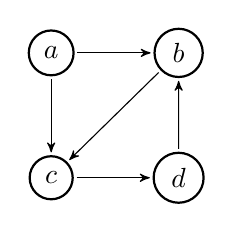
\begin{tikzpicture}
        \node[candidate] (a) [] {{$a$}};
        \node[candidate] (b) [right=of a] {{$b$}};
        \node[candidate] (c) [below=of a] {{$c$}};
        \node[candidate] (d) [right=of c] {{$d$}};

        \path[->] (a) edge (b);
        \path[->] (a) edge (c);
        \path[->] (b) edge (c);
        \path[->] (c) edge (d);
        \path[->] (d) edge (b);
    \end{tikzpicture}
\end{center}

In the case above, $a$ is the Condorcet winner in $\profile$. But $a,d$ are both Condorcet winners in $\profile_{-c}$. Since $F(\profile) \subseteq \{a,c\}$, we are not sure whether $a \in F(\profile)$. Applying such situation to another profile may cause $a$ not being a Condorcetian candidate.\footnote{But as we can see in above case, $a$ is still a Condorcetian candidate since $a \in F(\profile_{-b})$, and what Yifeng Ding want to show is $b$ is not Condorcetian (I guess), so maybe there's no such question\dots}

\part{Axiomatic Characterization of Split Cycle}
\chapter{Just Notes}

Two different types of function: 
\begin{itemize}
    \item \emph{Variable-election collective choice rule} (VCCR): output `defeat' relation (an \emph{asymmetric binary relation}).
    \item \emph{Variable-election social choice correspondence} (VSCC): output a set of undefeated candidates.
\end{itemize}

Another type of social choice function is \emph{variable-election social welfare function}, whose output is a strict weak order.

Acyclic VCCR `induces a VSCC that returns for a given profile $\profile$ the maximal (undefeated) elements of $f (\profile)$.'

The definition of Ranked Pairs as a VCCR somehow related to the proof of Theorem 5.39 in \textcite{Holliday2020} (?).


\printbibliography
\end{document}